% Final exam. Build both versions with ../build_pdfs.sh, or by hand:
%   pdflatex final_exam.tex                                                    -> exam for students
%   pdflatex -jobname=final_exam_solutions "\def\withsolutions{}% Final exam. Build both versions with ../build_pdfs.sh, or by hand:
%   pdflatex final_exam.tex                                                    -> exam for students
%   pdflatex -jobname=final_exam_solutions "\def\withsolutions{}% Final exam. Build both versions with ../build_pdfs.sh, or by hand:
%   pdflatex final_exam.tex                                                    -> exam for students
%   pdflatex -jobname=final_exam_solutions "\def\withsolutions{}% Final exam. Build both versions with ../build_pdfs.sh, or by hand:
%   pdflatex final_exam.tex                                                    -> exam for students
%   pdflatex -jobname=final_exam_solutions "\def\withsolutions{}\input{final_exam}"   -> answer key
\documentclass[11pt,a4paper,addpoints]{exam}
\ifdefined\withsolutions\printanswers\fi
\usepackage[T1]{fontenc}
\usepackage{lmodern}
\usepackage[margin=2.2cm]{geometry}
\usepackage{booktabs, array, amsmath, xcolor, tikz, multirow}
\usetikzlibrary{arrows.meta, positioning}
\input{../slides/figures/numbers.tex}
\definecolor{ocean}{HTML}{0D366B}
\renewcommand{\solutiontitle}{\noindent\textbf{\color{ocean}Model answer:}\enspace}
\SolutionEmphasis{\color{ocean!80!black}}
\shadedsolutions
\definecolor{SolutionColor}{HTML}{EAF2FC}
\pointsinrightmargin
% blank space for writing in the student version only; the answer key stays compact
\newcommand{\answerspace}[1]{\ifprintanswers\medskip\else\vspace{#1}\fi}
\newcommand{\qbreak}{\ifprintanswers\else\newpage\fi}
\bracketedpoints
\qformat{\textbf{Question \thequestion}\quad(\totalpoints\ points)\hfill}
\firstpageheader{Can a computer identify deep-sea animals?}{}{Final exam\ifprintanswers\ -- \textbf{ANSWER KEY}\fi}
\runningheader{}{}{Final exam\ifprintanswers\ -- answer key\fi}
\firstpagefooter{}{Page \thepage\ of \numpages}{}
\runningfooter{}{Page \thepage\ of \numpages}{}

\begin{document}
\begin{center}
{\LARGE\bfseries Final exam}\\[4pt]
{\large Can a computer identify deep-sea animals? -- A classifier project with FathomNet 2025}\\[10pt]
\end{center}

\noindent\begin{tabular}{@{}p{0.55\textwidth}p{0.4\textwidth}@{}}
Name: \hrulefill & Student ID: \hrulefill \\
\end{tabular}

\vspace{8pt}
\noindent\textbf{Time:} 90 minutes. \textbf{Allowed:} pocket calculator, one handwritten A4 sheet (both sides).
Answer in the space provided; short, precise answers are best. Give one decimal place for percentages.
There are \numpoints\ points in total.

\begin{center}
\gradetable[h][questions]
\end{center}

\begin{questions}

% =====================================================================  A
\question \textbf{Concepts.} Answer each part in one or two sentences.
\begin{parts}
\part[2] What is the difference between the \emph{training set} and the \emph{test set}?
\begin{solution}The training set is the set of labelled examples the classifier learns its rule from. The test set holds other labelled examples that are used only to measure how well the finished rule works on specimens it has not seen.\end{solution}
\answerspace{1.8cm}

\part[2] What is a \emph{feature}? Give two examples of features used in this course.
\begin{solution}A number that describes an object and is given to the classifier (like a character in a key). Examples: redness, brightness, edge strength, a pixel value, one of the 512 CNN embedding numbers.\end{solution}
\answerspace{1.8cm}

\part[2] Why is the accuracy on the training set not a good measure of how good a classifier is?
\begin{solution}A flexible classifier can memorise the training examples (e.g.\ 1-NN is always 100\,\% right on them). Training accuracy measures memory, not the ability to label new specimens; flexible rules can overfit.\end{solution}
\answerspace{1.8cm}

\part[2] There are 79 labels, each with the same number of test crops. What accuracy does the \emph{majority baseline} reach, and why is this number useful?
\begin{solution}$1/79 \approx 1.3\,\%$. Any real classifier must beat it; it tells you what ``no skill'' looks like (the baseline is much higher when labels are imbalanced or there are few of them).\end{solution}
\answerspace{1.8cm}

\part[2] Which classifier corresponds to a dichotomous identification key, and which to ``compare the specimen with the most similar ones in the reference collection''?
\begin{solution}Decision tree $=$ key; $k$-nearest neighbours $=$ comparing with the reference collection.\end{solution}
\answerspace{1.6cm}

\part[2] What does \emph{transfer learning} mean in this course?
\begin{solution}We used a CNN that was trained on a different task (ImageNet everyday photos) as a ready-made feature extractor for deep-sea crops, and trained only a simple classifier on its 512 output numbers.\end{solution}
\answerspace{1.8cm}

\part[2] What is the \emph{validation set} used for, and why must the test set not be used for the same purpose?
\begin{solution}For choosing between ideas/settings (features, classifier, $k$ \dots). If we chose on the test set, we would pick the idea that was lucky on those test crops and the reported score would be too optimistic.\end{solution}
\answerspace{1.8cm}

\part[2] Before using $k$-nearest neighbours we \emph{standardise} the features (each feature gets mean 0 and standard deviation 1). Why?
\begin{solution}$k$-NN uses distances. Without standardisation, a feature with large numbers (e.g.\ a value 0--255) dominates the distance and features with small ranges (0--1) are effectively ignored.\end{solution}
\answerspace{1.8cm}

\part[2] For the label \emph{Asteroidea} the classifier has high recall but low precision. Describe in words what it does.
\begin{solution}It finds almost all real sea stars, but it also calls many other animals ``Asteroidea'' -- many of its Asteroidea predictions are wrong.\end{solution}
\answerspace{1.8cm}

\part[2] Give two reasons why a label at a high rank (e.g.\ the class \emph{Asteroidea}) is harder to learn than a species label.
\begin{solution}(1) It covers many different-looking species, so its crops are very variable. (2) Experts use coarse labels exactly when the animal is hard to see (small, blurry, partly hidden), so the crops are of lower quality. (Also: it overlaps visually with its own lower-rank labels.)\end{solution}
\answerspace{1.8cm}
\end{parts}

% =====================================================================  B
\qbreak
\question \textbf{Accuracy, precision, recall.} A classifier was tested on 100 crops of three labels. Rows are the \emph{true} labels, columns the \emph{predicted} labels.
\begin{center}
\begin{tabular}{ll|ccc|c}
\toprule
 & & \multicolumn{3}{c|}{\textbf{predicted}} & \\
 & & Asteroidea & Ophiuroidea & Actiniaria & total \\
\midrule
\multirow{3}{*}{\textbf{true}} & Asteroidea (sea stars) & 40 & 8 & 2 & 50 \\
 & Ophiuroidea (brittle stars) & 10 & 25 & 5 & 40 \\
 & Actiniaria (sea anemones) & 0 & 5 & 5 & 10 \\
\midrule
 & total & 50 & 38 & 12 & 100 \\
\bottomrule
\end{tabular}
\end{center}
\begin{parts}
\part[3] Compute the accuracy.
\begin{solution}$(40+25+5)/100 = 70.0\,\%$.\end{solution}
\answerspace{1.3cm}
\part[6] Compute the recall of each label and the balanced accuracy.
\begin{solution}Asteroidea $40/50 = 80.0\,\%$; Ophiuroidea $25/40 = 62.5\,\%$; Actiniaria $5/10 = 50.0\,\%$. Balanced accuracy $= (80.0+62.5+50.0)/3 = 64.2\,\%$.\end{solution}
\answerspace{2.1cm}
\part[4] Compute the precision of \emph{Actiniaria} and of \emph{Ophiuroidea}.
\begin{solution}Actiniaria: $5/12 = 41.7\,\%$. Ophiuroidea: $25/38 = 65.8\,\%$.\end{solution}
\answerspace{1.6cm}
\part[3] What accuracy and what balanced accuracy would the majority baseline reach on these 100 crops?
\begin{solution}It always predicts Asteroidea: accuracy $50/100 = 50.0\,\%$; recalls 100, 0, 0\,\% $\Rightarrow$ balanced accuracy $33.3\,\%$.\end{solution}
\answerspace{1.6cm}
\part[4] Asteroidea and Ophiuroidea are both Echinodermata; Actiniaria are Cnidaria. How many of the 30 mistakes stay within the correct phylum? Which kind of mistake is worse for a biodiversity survey, and why?
\begin{solution}Within Echinodermata: $8 + 10 = 18$ of 30 (60\,\%); the other 12 confuse phyla. A cross-phylum mistake is worse: it puts the animal in a completely different part of the tree of life (different body plan, ecology, feeding), so higher-rank summaries (e.g.\ ``number of echinoderms'') become wrong too; a within-phylum mistake still gives correct counts at phylum level.\end{solution}
\answerspace{2.1cm}
\end{parts}

% =====================================================================  C
\qbreak
\question \textbf{Classifiers by hand.}
Six training crops are described by two standardised features (redness, brightness):
\begin{center}
\begin{tabular}{cccl}
\toprule
crop & redness & brightness & label \\
\midrule
1 & 2 & 8 & \emph{Pyrosoma} (tunicate) \\
2 & 1 & 6 & \emph{Pyrosoma} \\
3 & 3 & 5 & \emph{Pyrosoma} \\
4 & 7 & 4 & \emph{Ptychogastria} (jellyfish) \\
5 & 8 & 7 & \emph{Ptychogastria} \\
6 & 6 & 2 & \emph{Ptychogastria} \\
\bottomrule
\end{tabular}
\end{center}
A new crop $X$ has redness 5 and brightness 5.
\begin{parts}
\part[6] Compute the Euclidean distance from $X$ to each training crop
\\ \hspace*{1.5em}$d = \sqrt{(\Delta\,\text{redness})^2 + (\Delta\,\text{brightness})^2}$
\begin{solution}1: $\sqrt{9+9}=4.24$; 2: $\sqrt{16+1}=4.12$; 3: $\sqrt{4+0}=2.00$; 4: $\sqrt{4+1}=2.24$; 5: $\sqrt{9+4}=3.61$; 6: $\sqrt{1+9}=3.16$.\end{solution}
\answerspace{2.6cm}
\part[4] Classify $X$ with $k$-NN for $k = 1$ and for $k = 3$. Why can the two answers differ?
\begin{solution}$k=1$: nearest is crop 3 $\Rightarrow$ \emph{Pyrosoma}. $k=3$: crops 3 (P), 4 (J), 6 (J) $\Rightarrow$ \emph{Ptychogastria} (2:1). A single neighbour can be an unusual specimen; a vote over more neighbours smooths the boundary (less sensitive to single crops, less overfitting).\end{solution}
\answerspace{2.1cm}
\part[4] Classify $X$ with the nearest-centroid classifier. Show the two centroids.
\begin{solution}Centroid \emph{Pyrosoma} $=(2,\ 6.33)$, \emph{Ptychogastria} $=(7,\ 4.33)$. Distances: $\sqrt{9+1.78}=3.28$ and $\sqrt{4+0.44}=2.11$ $\Rightarrow$ \emph{Ptychogastria}.\end{solution}
\answerspace{2.1cm}
\part[3] A decision tree learned from crops of four labels:
\begin{center}
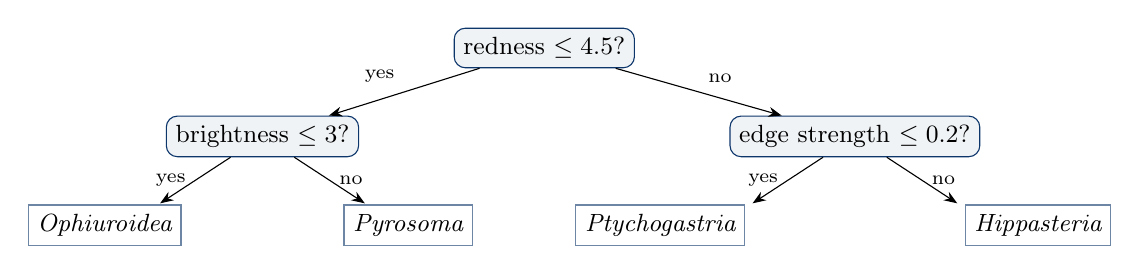
\begin{tikzpicture}[>=Stealth, font=\small, node distance=6mm and 4mm,
  q/.style={draw=ocean, rounded corners, fill=ocean!6, align=center},
  l/.style={draw=ocean!60, fill=white, align=center, font=\small\itshape}]
  \node[q] (r) {redness $\le 4.5$?};
  \node[q, below left=of r, xshift=-8mm] (a) {brightness $\le 3$?};
  \node[q, below right=of r, xshift=8mm] (b) {edge strength $\le 0.2$?};
  \node[l, below left=of a, xshift=6mm] {Ophiuroidea};
  \node[l, below right=of a, xshift=-6mm] {Pyrosoma};
  \node[l, below left=of b, xshift=6mm] {Ptychogastria};
  \node[l, below right=of b, xshift=-6mm] {Hippasteria};
  \draw[->] (r) -- node[above left, font=\scriptsize]{yes} (a);
  \draw[->] (r) -- node[above right, font=\scriptsize]{no} (b);
  \draw[->] (a) -- node[left, font=\scriptsize]{yes} +(-1.3,-0.85);
  \draw[->] (a) -- node[right, font=\scriptsize]{no} +(1.3,-0.85);
  \draw[->] (b) -- node[left, font=\scriptsize]{yes} +(-1.3,-0.85);
  \draw[->] (b) -- node[right, font=\scriptsize]{no} +(1.3,-0.85);
\end{tikzpicture}
\end{center}
Classify: (i) redness 6, brightness 2, edge strength 0.35; (ii) redness 3, brightness 7, edge strength 0.1; (iii) redness 4.5, brightness 2.5, edge strength 0.5.
\begin{solution}(i) $6 > 4.5$ $\rightarrow$ edge $0.35 > 0.2$ $\rightarrow$ \emph{Hippasteria}. (ii) $3 \le 4.5$ $\rightarrow$ brightness $7 > 3$ $\rightarrow$ \emph{Pyrosoma}. (iii) $4.5 \le 4.5$ $\rightarrow$ brightness $2.5 \le 3$ $\rightarrow$ \emph{Ophiuroidea}.\end{solution}
\answerspace{1.6cm}
\part[3] A colleague grows the tree until every leaf contains exactly one training crop. What happens to the training accuracy and to the test accuracy? Use the comparison with a taxonomist's key.
\begin{solution}Training accuracy becomes (nearly) 100\,\%, test accuracy usually drops: the tree overfits. It is like a key with one couplet per museum specimen -- it describes the individual specimens (and their noise) instead of the characters of the species, so new specimens fall into the wrong leaves.\end{solution}
\answerspace{2.1cm}
\end{parts}

% =====================================================================  D
\qbreak
\question \textbf{Interpreting an experiment.} The reference run of this course used CNN features (ResNet-18) and all \RefCrops\ crops, 79 labels, and three ways of splitting them into 75\,\% training and 25\,\% test crops (mean of 3 repetitions):
\begin{center}
\begin{tabular}{lcccc}
\toprule
 & \multicolumn{2}{c}{logistic regression} & \multicolumn{2}{c}{5-nearest neighbours} \\
split & train acc. & test acc. & train acc. & test acc. \\
\midrule
random (crop by crop) & \RefTrainLogregRandom & \RefRandomAcc & \RefTrainKnnRandom & \RefRandomAccKnn \\
image (crops of a frame together) & \RefTrainLogregImage & \RefImageAcc & \RefTrainKnnImage & \RefImageAccKnn \\
dive (crops of a dive together) & \RefTrainLogregDive & \RefDiveAcc & \RefTrainKnnDive & \RefDiveAccKnn \\
\bottomrule
\end{tabular}
\end{center}
In the random split, \RefSeenDiveRandom\ of the test crops come from a dive that also contributed training crops; in the dive split, 0\,\%.
\begin{parts}
\part[4] Describe the main result in two sentences.
\begin{solution}With the same features and classifier, test accuracy drops strongly from the random split (\RefRandomAcc) to the dive split (\RefDiveAcc), while training accuracy stays high. Keeping whole images together changes little; keeping whole dives together changes a lot.\end{solution}
\answerspace{2.1cm}
\part[6] Explain \emph{why} the accuracy depends on the split. Use what you know about how the images were recorded.
\begin{solution}Frames of one dive are recorded within hours at one site, with the same camera, light and background, and often show the same individual animal several times. In a random split near-identical crops land in training and test, so the classifier can ``recognise'' a crop it has practically seen (data leakage). In a dive split the test animals come from other places, other individuals, other conditions -- the classifier must really generalise.\end{solution}
\answerspace{3.1cm}
\part[3] $k$-NN profits more from the random split than logistic regression. Suggest a reason.
\begin{solution}$k$-NN labels a crop by its most similar training crops; with a random split these are often frames of the same individual from the same dive, so it effectively looks up a near-duplicate. Logistic regression learns one smooth weighted rule per label and relies less on individual training crops.\end{solution}
\answerspace{1.8cm}
\part[3] Which test accuracy belongs in a report about using the classifier on a future expedition? Justify.
\begin{solution}The dive-split number: a future expedition consists of new dives, so only a test on unseen dives estimates that situation; the random-split number is inflated by leakage.\end{solution}
\answerspace{1.8cm}
\part[4] A newspaper writes: ``AI identifies deep-sea animals with 98\,\% accuracy -- taxonomists no longer needed.'' Give two critical questions you would ask.
\begin{solution}Any two, e.g.: Was the 98\,\% measured on images from new dives/sites or on frames similar to the training images? Accuracy on which labels -- species or coarse groups, and how good is it on rare ones (balanced accuracy)? How severe are the remaining mistakes? Who labelled the test data -- are the labels themselves checked? Is it better than a sensible baseline? (The FathomNet winners: $\approx$98\,\% on training images but only 57--61\,\% on new dives.)\end{solution}
\answerspace{2.3cm}
\end{parts}

% =====================================================================  E
\qbreak
\question \textbf{Mistakes in the tree of life.}
\begin{center}
\small
\begin{tabular}{llllll}
\toprule
label & phylum & class & order & family & genus \\
\midrule
\emph{Sebastes diploproa} (species) & Chordata & Teleostei & Perciformes & Sebastidae & \emph{Sebastes} \\
\emph{Sebastes} (genus) & Chordata & Teleostei & Perciformes & Sebastidae & \emph{Sebastes} \\
\emph{Sebastolobus} (genus) & Chordata & Teleostei & Perciformes & Sebastidae & \emph{Sebastolobus} \\
Asteroidea (class) & Echinodermata & Asteroidea & & & \\
Ophiuroidea (class) & Echinodermata & Ophiuroidea & & & \\
Actiniaria (order) & Cnidaria & Hexacorallia & Actiniaria & & \\
\bottomrule
\end{tabular}
\end{center}
The \emph{tree distance} is the number of steps from the true label up to the lowest rank both labels share, plus the steps down to the predicted label (ranks: kingdom, phylum, class, order, family, genus, species).
\begin{parts}
\part[6] For each mistake give the lowest shared rank and the tree distance:
(i) truth \emph{Sebastes}, prediction \emph{Sebastes diploproa};
(ii) truth \emph{Sebastes diploproa}, prediction \emph{Sebastolobus};
(iii) truth Asteroidea, prediction Ophiuroidea;
(iv) truth Asteroidea, prediction Actiniaria.
\begin{solution}(i) genus \emph{Sebastes}: $0 + 1 = 1$. (ii) family Sebastidae: $2 + 1 = 3$ (species$\to$genus$\to$family, family$\to$genus). (iii) phylum Echinodermata: $1 + 1 = 2$. (iv) kingdom Animalia: $2 + 3 = 5$.\end{solution}
\answerspace{2.9cm}
\part[4] Mistake (i) is often not the classifier's fault. Explain why, and say what this means for how we should score such predictions.
\begin{solution}\emph{Sebastes diploproa} is a species inside the genus \emph{Sebastes}; a crop labelled \emph{Sebastes} may well show a \emph{S.\ diploproa} that the annotator could not identify to species. The prediction is then possibly correct but more specific than the label. A plain right/wrong score punishes this as hard as a cross-phylum error; a taxonomic distance (or scoring at genus rank) treats it as the small or non-mistake it is.\end{solution}
\answerspace{2.3cm}
\end{parts}

% =====================================================================  F
\qbreak
\question[10] \textbf{Design.} A research group wants to use a classifier to count animals in 200 hours of new ROV video from a seamount that has never been surveyed. They have the FathomNet training data. Describe in 6--10 bullet points how you would build, test and use the classifier responsibly.
\begin{solution}Credit for (about 1 point each, max.\ 10):
\begin{itemize}
\item Features from a pretrained CNN (transfer learning), classifier such as logistic regression; possibly fine-tune.
\item Split train/validation/test \textbf{by dive} (or by site/cruise); tune on validation only; test once.
\item Better still: annotate a small sample of the new seamount video by experts and test on it (new site, possibly new camera).
\item Compare with the majority baseline; report balanced accuracy / macro-F1, not only accuracy.
\item Per-label recall: find which taxa are unreliable; report those at a coarser rank or check by hand.
\item Look at mistake severity in the tree of life; report counts at the rank where the classifier is reliable (e.g.\ phylum/class).
\item Animals or labels not in the 79 training labels will be forced into a wrong label -- plan for ``unknown''.
\item Use the confidence: let experts check low-confidence predictions, and a random sample of confident ones (confident mistakes exist).
\item Look at mistakes with images; some are label errors; tiny/blurry crops are unreliable.
\item Document data, split, metrics and limitations; acknowledge FathomNet.
\end{itemize}\end{solution}
\answerspace{9.1cm}
\end{questions}
\end{document}
"   -> answer key
\documentclass[11pt,a4paper,addpoints]{exam}
\ifdefined\withsolutions\printanswers\fi
\usepackage[T1]{fontenc}
\usepackage{lmodern}
\usepackage[margin=2.2cm]{geometry}
\usepackage{booktabs, array, amsmath, xcolor, tikz, multirow}
\usetikzlibrary{arrows.meta, positioning}
% generated by write_numbers.py from results/reference_results.json - do not edit
\newcommand{\RefCrops}{23{,}664}
\newcommand{\RefDives}{1{,}465}
\newcommand{\RefTopTenDives}{21\,\%}
\newcommand{\RefTwoTrain}{444}
\newcommand{\RefTwoTest}{148}
\newcommand{\RefThr}{0.05}
\newcommand{\RefThrTrain}{98.4\,\%}
\newcommand{\RefThrTest}{98.0\,\%}
\newcommand{\RefCSPhylumMajority}{30.4\,\%}
\newcommand{\RefCSPhylumCentroid}{26.4\,\%}
\newcommand{\RefCSPhylumKnn}{55.0\,\%}
\newcommand{\RefCSPhylumTree}{50.3\,\%}
\newcommand{\RefCSLabelMajority}{1.3\,\%}
\newcommand{\RefCSLabelCentroid}{15.9\,\%}
\newcommand{\RefCSLabelKnn}{33.6\,\%}
\newcommand{\RefCSLabelTree}{23.7\,\%}
\newcommand{\RefCSLabelBest}{33.6\,\%}
\newcommand{\RefZooBestName}{neural network (MLP)}
\newcommand{\RefZooBest}{64.6\,\%}
\newcommand{\RefZooBestPixels}{46.3\,\%}
\newcommand{\RefZooBestColour}{48.4\,\%}
\newcommand{\RefZooRows}{majority baseline & 1.3\,\% & 1.3\,\% & $<$1\,s \\
nearest centroid & 39.9\,\% & 37.9\,\% & 2\,s \\
5-nearest neighbours & 69.9\,\% & 53.4\,\% & $<$1\,s \\
decision tree & 100.0\,\% & 20.5\,\% & 48\,s \\
random forest & 100.0\,\% & 56.1\,\% & 93\,s \\
logistic regression & 90.7\,\% & 63.7\,\% & 21\,s \\
neural network (MLP) & 92.4\,\% & 64.6\,\% & 13\,s \\}
\newcommand{\RefRandomAcc}{63.5\,\%}
\newcommand{\RefRandomAccKnn}{53.5\,\%}
\newcommand{\RefTrainLogregRandom}{90.7\,\%}
\newcommand{\RefTrainKnnRandom}{70.0\,\%}
\newcommand{\RefImageAcc}{57.5\,\%}
\newcommand{\RefImageAccKnn}{45.5\,\%}
\newcommand{\RefTrainLogregImage}{91.1\,\%}
\newcommand{\RefTrainKnnImage}{71.0\,\%}
\newcommand{\RefDiveAcc}{49.6\,\%}
\newcommand{\RefDiveAccKnn}{35.5\,\%}
\newcommand{\RefTrainLogregDive}{91.0\,\%}
\newcommand{\RefTrainKnnDive}{71.6\,\%}
\newcommand{\RefSeenDiveRandom}{97\,\%}
\newcommand{\RefRecallRows}{species & 33 & 67\,\% \\
genus & 21 & 69\,\% \\
family & 8 & 64\,\% \\
order & 6 & 56\,\% \\
class & 6 & 44\,\% \\
phylum & 1 & 27\,\% \\
other rank & 4 & 58\,\% \\}
\newcommand{\RefSevKingdom}{55\,\%}
\newcommand{\RefSevNear}{21\,\%}
\newcommand{\RefRandPhylumAcc}{80.0\,\%}
\newcommand{\RefDivePhylumAcc}{72.6\,\%}
\newcommand{\RefDiveFone}{0.475}
\newcommand{\RefDiveAccSingle}{49.8\,\%}

\definecolor{ocean}{HTML}{0D366B}
\renewcommand{\solutiontitle}{\noindent\textbf{\color{ocean}Model answer:}\enspace}
\SolutionEmphasis{\color{ocean!80!black}}
\shadedsolutions
\definecolor{SolutionColor}{HTML}{EAF2FC}
\pointsinrightmargin
% blank space for writing in the student version only; the answer key stays compact
\newcommand{\answerspace}[1]{\ifprintanswers\medskip\else\vspace{#1}\fi}
\newcommand{\qbreak}{\ifprintanswers\else\newpage\fi}
\bracketedpoints
\qformat{\textbf{Question \thequestion}\quad(\totalpoints\ points)\hfill}
\firstpageheader{Can a computer identify deep-sea animals?}{}{Final exam\ifprintanswers\ -- \textbf{ANSWER KEY}\fi}
\runningheader{}{}{Final exam\ifprintanswers\ -- answer key\fi}
\firstpagefooter{}{Page \thepage\ of \numpages}{}
\runningfooter{}{Page \thepage\ of \numpages}{}

\begin{document}
\begin{center}
{\LARGE\bfseries Final exam}\\[4pt]
{\large Can a computer identify deep-sea animals? -- A classifier project with FathomNet 2025}\\[10pt]
\end{center}

\noindent\begin{tabular}{@{}p{0.55\textwidth}p{0.4\textwidth}@{}}
Name: \hrulefill & Student ID: \hrulefill \\
\end{tabular}

\vspace{8pt}
\noindent\textbf{Time:} 90 minutes. \textbf{Allowed:} pocket calculator, one handwritten A4 sheet (both sides).
Answer in the space provided; short, precise answers are best. Give one decimal place for percentages.
There are \numpoints\ points in total.

\begin{center}
\gradetable[h][questions]
\end{center}

\begin{questions}

% =====================================================================  A
\question \textbf{Concepts.} Answer each part in one or two sentences.
\begin{parts}
\part[2] What is the difference between the \emph{training set} and the \emph{test set}?
\begin{solution}The training set is the set of labelled examples the classifier learns its rule from. The test set holds other labelled examples that are used only to measure how well the finished rule works on specimens it has not seen.\end{solution}
\answerspace{1.8cm}

\part[2] What is a \emph{feature}? Give two examples of features used in this course.
\begin{solution}A number that describes an object and is given to the classifier (like a character in a key). Examples: redness, brightness, edge strength, a pixel value, one of the 512 CNN embedding numbers.\end{solution}
\answerspace{1.8cm}

\part[2] Why is the accuracy on the training set not a good measure of how good a classifier is?
\begin{solution}A flexible classifier can memorise the training examples (e.g.\ 1-NN is always 100\,\% right on them). Training accuracy measures memory, not the ability to label new specimens; flexible rules can overfit.\end{solution}
\answerspace{1.8cm}

\part[2] There are 79 labels, each with the same number of test crops. What accuracy does the \emph{majority baseline} reach, and why is this number useful?
\begin{solution}$1/79 \approx 1.3\,\%$. Any real classifier must beat it; it tells you what ``no skill'' looks like (the baseline is much higher when labels are imbalanced or there are few of them).\end{solution}
\answerspace{1.8cm}

\part[2] Which classifier corresponds to a dichotomous identification key, and which to ``compare the specimen with the most similar ones in the reference collection''?
\begin{solution}Decision tree $=$ key; $k$-nearest neighbours $=$ comparing with the reference collection.\end{solution}
\answerspace{1.6cm}

\part[2] What does \emph{transfer learning} mean in this course?
\begin{solution}We used a CNN that was trained on a different task (ImageNet everyday photos) as a ready-made feature extractor for deep-sea crops, and trained only a simple classifier on its 512 output numbers.\end{solution}
\answerspace{1.8cm}

\part[2] What is the \emph{validation set} used for, and why must the test set not be used for the same purpose?
\begin{solution}For choosing between ideas/settings (features, classifier, $k$ \dots). If we chose on the test set, we would pick the idea that was lucky on those test crops and the reported score would be too optimistic.\end{solution}
\answerspace{1.8cm}

\part[2] Before using $k$-nearest neighbours we \emph{standardise} the features (each feature gets mean 0 and standard deviation 1). Why?
\begin{solution}$k$-NN uses distances. Without standardisation, a feature with large numbers (e.g.\ a value 0--255) dominates the distance and features with small ranges (0--1) are effectively ignored.\end{solution}
\answerspace{1.8cm}

\part[2] For the label \emph{Asteroidea} the classifier has high recall but low precision. Describe in words what it does.
\begin{solution}It finds almost all real sea stars, but it also calls many other animals ``Asteroidea'' -- many of its Asteroidea predictions are wrong.\end{solution}
\answerspace{1.8cm}

\part[2] Give two reasons why a label at a high rank (e.g.\ the class \emph{Asteroidea}) is harder to learn than a species label.
\begin{solution}(1) It covers many different-looking species, so its crops are very variable. (2) Experts use coarse labels exactly when the animal is hard to see (small, blurry, partly hidden), so the crops are of lower quality. (Also: it overlaps visually with its own lower-rank labels.)\end{solution}
\answerspace{1.8cm}
\end{parts}

% =====================================================================  B
\qbreak
\question \textbf{Accuracy, precision, recall.} A classifier was tested on 100 crops of three labels. Rows are the \emph{true} labels, columns the \emph{predicted} labels.
\begin{center}
\begin{tabular}{ll|ccc|c}
\toprule
 & & \multicolumn{3}{c|}{\textbf{predicted}} & \\
 & & Asteroidea & Ophiuroidea & Actiniaria & total \\
\midrule
\multirow{3}{*}{\textbf{true}} & Asteroidea (sea stars) & 40 & 8 & 2 & 50 \\
 & Ophiuroidea (brittle stars) & 10 & 25 & 5 & 40 \\
 & Actiniaria (sea anemones) & 0 & 5 & 5 & 10 \\
\midrule
 & total & 50 & 38 & 12 & 100 \\
\bottomrule
\end{tabular}
\end{center}
\begin{parts}
\part[3] Compute the accuracy.
\begin{solution}$(40+25+5)/100 = 70.0\,\%$.\end{solution}
\answerspace{1.3cm}
\part[6] Compute the recall of each label and the balanced accuracy.
\begin{solution}Asteroidea $40/50 = 80.0\,\%$; Ophiuroidea $25/40 = 62.5\,\%$; Actiniaria $5/10 = 50.0\,\%$. Balanced accuracy $= (80.0+62.5+50.0)/3 = 64.2\,\%$.\end{solution}
\answerspace{2.1cm}
\part[4] Compute the precision of \emph{Actiniaria} and of \emph{Ophiuroidea}.
\begin{solution}Actiniaria: $5/12 = 41.7\,\%$. Ophiuroidea: $25/38 = 65.8\,\%$.\end{solution}
\answerspace{1.6cm}
\part[3] What accuracy and what balanced accuracy would the majority baseline reach on these 100 crops?
\begin{solution}It always predicts Asteroidea: accuracy $50/100 = 50.0\,\%$; recalls 100, 0, 0\,\% $\Rightarrow$ balanced accuracy $33.3\,\%$.\end{solution}
\answerspace{1.6cm}
\part[4] Asteroidea and Ophiuroidea are both Echinodermata; Actiniaria are Cnidaria. How many of the 30 mistakes stay within the correct phylum? Which kind of mistake is worse for a biodiversity survey, and why?
\begin{solution}Within Echinodermata: $8 + 10 = 18$ of 30 (60\,\%); the other 12 confuse phyla. A cross-phylum mistake is worse: it puts the animal in a completely different part of the tree of life (different body plan, ecology, feeding), so higher-rank summaries (e.g.\ ``number of echinoderms'') become wrong too; a within-phylum mistake still gives correct counts at phylum level.\end{solution}
\answerspace{2.1cm}
\end{parts}

% =====================================================================  C
\qbreak
\question \textbf{Classifiers by hand.}
Six training crops are described by two standardised features (redness, brightness):
\begin{center}
\begin{tabular}{cccl}
\toprule
crop & redness & brightness & label \\
\midrule
1 & 2 & 8 & \emph{Pyrosoma} (tunicate) \\
2 & 1 & 6 & \emph{Pyrosoma} \\
3 & 3 & 5 & \emph{Pyrosoma} \\
4 & 7 & 4 & \emph{Ptychogastria} (jellyfish) \\
5 & 8 & 7 & \emph{Ptychogastria} \\
6 & 6 & 2 & \emph{Ptychogastria} \\
\bottomrule
\end{tabular}
\end{center}
A new crop $X$ has redness 5 and brightness 5.
\begin{parts}
\part[6] Compute the Euclidean distance from $X$ to each training crop
\\ \hspace*{1.5em}$d = \sqrt{(\Delta\,\text{redness})^2 + (\Delta\,\text{brightness})^2}$
\begin{solution}1: $\sqrt{9+9}=4.24$; 2: $\sqrt{16+1}=4.12$; 3: $\sqrt{4+0}=2.00$; 4: $\sqrt{4+1}=2.24$; 5: $\sqrt{9+4}=3.61$; 6: $\sqrt{1+9}=3.16$.\end{solution}
\answerspace{2.6cm}
\part[4] Classify $X$ with $k$-NN for $k = 1$ and for $k = 3$. Why can the two answers differ?
\begin{solution}$k=1$: nearest is crop 3 $\Rightarrow$ \emph{Pyrosoma}. $k=3$: crops 3 (P), 4 (J), 6 (J) $\Rightarrow$ \emph{Ptychogastria} (2:1). A single neighbour can be an unusual specimen; a vote over more neighbours smooths the boundary (less sensitive to single crops, less overfitting).\end{solution}
\answerspace{2.1cm}
\part[4] Classify $X$ with the nearest-centroid classifier. Show the two centroids.
\begin{solution}Centroid \emph{Pyrosoma} $=(2,\ 6.33)$, \emph{Ptychogastria} $=(7,\ 4.33)$. Distances: $\sqrt{9+1.78}=3.28$ and $\sqrt{4+0.44}=2.11$ $\Rightarrow$ \emph{Ptychogastria}.\end{solution}
\answerspace{2.1cm}
\part[3] A decision tree learned from crops of four labels:
\begin{center}
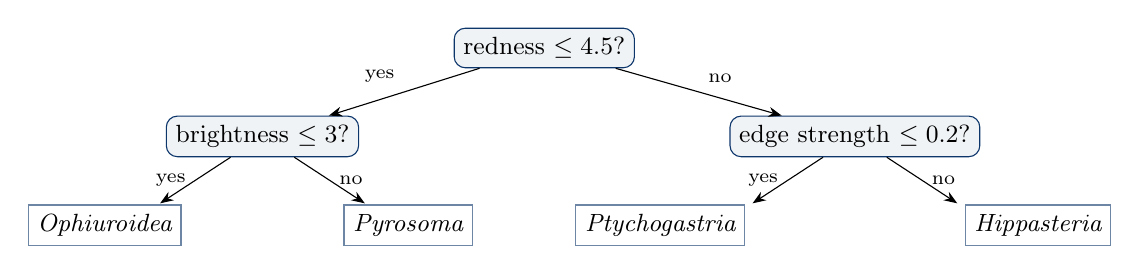
\begin{tikzpicture}[>=Stealth, font=\small, node distance=6mm and 4mm,
  q/.style={draw=ocean, rounded corners, fill=ocean!6, align=center},
  l/.style={draw=ocean!60, fill=white, align=center, font=\small\itshape}]
  \node[q] (r) {redness $\le 4.5$?};
  \node[q, below left=of r, xshift=-8mm] (a) {brightness $\le 3$?};
  \node[q, below right=of r, xshift=8mm] (b) {edge strength $\le 0.2$?};
  \node[l, below left=of a, xshift=6mm] {Ophiuroidea};
  \node[l, below right=of a, xshift=-6mm] {Pyrosoma};
  \node[l, below left=of b, xshift=6mm] {Ptychogastria};
  \node[l, below right=of b, xshift=-6mm] {Hippasteria};
  \draw[->] (r) -- node[above left, font=\scriptsize]{yes} (a);
  \draw[->] (r) -- node[above right, font=\scriptsize]{no} (b);
  \draw[->] (a) -- node[left, font=\scriptsize]{yes} +(-1.3,-0.85);
  \draw[->] (a) -- node[right, font=\scriptsize]{no} +(1.3,-0.85);
  \draw[->] (b) -- node[left, font=\scriptsize]{yes} +(-1.3,-0.85);
  \draw[->] (b) -- node[right, font=\scriptsize]{no} +(1.3,-0.85);
\end{tikzpicture}
\end{center}
Classify: (i) redness 6, brightness 2, edge strength 0.35; (ii) redness 3, brightness 7, edge strength 0.1; (iii) redness 4.5, brightness 2.5, edge strength 0.5.
\begin{solution}(i) $6 > 4.5$ $\rightarrow$ edge $0.35 > 0.2$ $\rightarrow$ \emph{Hippasteria}. (ii) $3 \le 4.5$ $\rightarrow$ brightness $7 > 3$ $\rightarrow$ \emph{Pyrosoma}. (iii) $4.5 \le 4.5$ $\rightarrow$ brightness $2.5 \le 3$ $\rightarrow$ \emph{Ophiuroidea}.\end{solution}
\answerspace{1.6cm}
\part[3] A colleague grows the tree until every leaf contains exactly one training crop. What happens to the training accuracy and to the test accuracy? Use the comparison with a taxonomist's key.
\begin{solution}Training accuracy becomes (nearly) 100\,\%, test accuracy usually drops: the tree overfits. It is like a key with one couplet per museum specimen -- it describes the individual specimens (and their noise) instead of the characters of the species, so new specimens fall into the wrong leaves.\end{solution}
\answerspace{2.1cm}
\end{parts}

% =====================================================================  D
\qbreak
\question \textbf{Interpreting an experiment.} The reference run of this course used CNN features (ResNet-18) and all \RefCrops\ crops, 79 labels, and three ways of splitting them into 75\,\% training and 25\,\% test crops (mean of 3 repetitions):
\begin{center}
\begin{tabular}{lcccc}
\toprule
 & \multicolumn{2}{c}{logistic regression} & \multicolumn{2}{c}{5-nearest neighbours} \\
split & train acc. & test acc. & train acc. & test acc. \\
\midrule
random (crop by crop) & \RefTrainLogregRandom & \RefRandomAcc & \RefTrainKnnRandom & \RefRandomAccKnn \\
image (crops of a frame together) & \RefTrainLogregImage & \RefImageAcc & \RefTrainKnnImage & \RefImageAccKnn \\
dive (crops of a dive together) & \RefTrainLogregDive & \RefDiveAcc & \RefTrainKnnDive & \RefDiveAccKnn \\
\bottomrule
\end{tabular}
\end{center}
In the random split, \RefSeenDiveRandom\ of the test crops come from a dive that also contributed training crops; in the dive split, 0\,\%.
\begin{parts}
\part[4] Describe the main result in two sentences.
\begin{solution}With the same features and classifier, test accuracy drops strongly from the random split (\RefRandomAcc) to the dive split (\RefDiveAcc), while training accuracy stays high. Keeping whole images together changes little; keeping whole dives together changes a lot.\end{solution}
\answerspace{2.1cm}
\part[6] Explain \emph{why} the accuracy depends on the split. Use what you know about how the images were recorded.
\begin{solution}Frames of one dive are recorded within hours at one site, with the same camera, light and background, and often show the same individual animal several times. In a random split near-identical crops land in training and test, so the classifier can ``recognise'' a crop it has practically seen (data leakage). In a dive split the test animals come from other places, other individuals, other conditions -- the classifier must really generalise.\end{solution}
\answerspace{3.1cm}
\part[3] $k$-NN profits more from the random split than logistic regression. Suggest a reason.
\begin{solution}$k$-NN labels a crop by its most similar training crops; with a random split these are often frames of the same individual from the same dive, so it effectively looks up a near-duplicate. Logistic regression learns one smooth weighted rule per label and relies less on individual training crops.\end{solution}
\answerspace{1.8cm}
\part[3] Which test accuracy belongs in a report about using the classifier on a future expedition? Justify.
\begin{solution}The dive-split number: a future expedition consists of new dives, so only a test on unseen dives estimates that situation; the random-split number is inflated by leakage.\end{solution}
\answerspace{1.8cm}
\part[4] A newspaper writes: ``AI identifies deep-sea animals with 98\,\% accuracy -- taxonomists no longer needed.'' Give two critical questions you would ask.
\begin{solution}Any two, e.g.: Was the 98\,\% measured on images from new dives/sites or on frames similar to the training images? Accuracy on which labels -- species or coarse groups, and how good is it on rare ones (balanced accuracy)? How severe are the remaining mistakes? Who labelled the test data -- are the labels themselves checked? Is it better than a sensible baseline? (The FathomNet winners: $\approx$98\,\% on training images but only 57--61\,\% on new dives.)\end{solution}
\answerspace{2.3cm}
\end{parts}

% =====================================================================  E
\qbreak
\question \textbf{Mistakes in the tree of life.}
\begin{center}
\small
\begin{tabular}{llllll}
\toprule
label & phylum & class & order & family & genus \\
\midrule
\emph{Sebastes diploproa} (species) & Chordata & Teleostei & Perciformes & Sebastidae & \emph{Sebastes} \\
\emph{Sebastes} (genus) & Chordata & Teleostei & Perciformes & Sebastidae & \emph{Sebastes} \\
\emph{Sebastolobus} (genus) & Chordata & Teleostei & Perciformes & Sebastidae & \emph{Sebastolobus} \\
Asteroidea (class) & Echinodermata & Asteroidea & & & \\
Ophiuroidea (class) & Echinodermata & Ophiuroidea & & & \\
Actiniaria (order) & Cnidaria & Hexacorallia & Actiniaria & & \\
\bottomrule
\end{tabular}
\end{center}
The \emph{tree distance} is the number of steps from the true label up to the lowest rank both labels share, plus the steps down to the predicted label (ranks: kingdom, phylum, class, order, family, genus, species).
\begin{parts}
\part[6] For each mistake give the lowest shared rank and the tree distance:
(i) truth \emph{Sebastes}, prediction \emph{Sebastes diploproa};
(ii) truth \emph{Sebastes diploproa}, prediction \emph{Sebastolobus};
(iii) truth Asteroidea, prediction Ophiuroidea;
(iv) truth Asteroidea, prediction Actiniaria.
\begin{solution}(i) genus \emph{Sebastes}: $0 + 1 = 1$. (ii) family Sebastidae: $2 + 1 = 3$ (species$\to$genus$\to$family, family$\to$genus). (iii) phylum Echinodermata: $1 + 1 = 2$. (iv) kingdom Animalia: $2 + 3 = 5$.\end{solution}
\answerspace{2.9cm}
\part[4] Mistake (i) is often not the classifier's fault. Explain why, and say what this means for how we should score such predictions.
\begin{solution}\emph{Sebastes diploproa} is a species inside the genus \emph{Sebastes}; a crop labelled \emph{Sebastes} may well show a \emph{S.\ diploproa} that the annotator could not identify to species. The prediction is then possibly correct but more specific than the label. A plain right/wrong score punishes this as hard as a cross-phylum error; a taxonomic distance (or scoring at genus rank) treats it as the small or non-mistake it is.\end{solution}
\answerspace{2.3cm}
\end{parts}

% =====================================================================  F
\qbreak
\question[10] \textbf{Design.} A research group wants to use a classifier to count animals in 200 hours of new ROV video from a seamount that has never been surveyed. They have the FathomNet training data. Describe in 6--10 bullet points how you would build, test and use the classifier responsibly.
\begin{solution}Credit for (about 1 point each, max.\ 10):
\begin{itemize}
\item Features from a pretrained CNN (transfer learning), classifier such as logistic regression; possibly fine-tune.
\item Split train/validation/test \textbf{by dive} (or by site/cruise); tune on validation only; test once.
\item Better still: annotate a small sample of the new seamount video by experts and test on it (new site, possibly new camera).
\item Compare with the majority baseline; report balanced accuracy / macro-F1, not only accuracy.
\item Per-label recall: find which taxa are unreliable; report those at a coarser rank or check by hand.
\item Look at mistake severity in the tree of life; report counts at the rank where the classifier is reliable (e.g.\ phylum/class).
\item Animals or labels not in the 79 training labels will be forced into a wrong label -- plan for ``unknown''.
\item Use the confidence: let experts check low-confidence predictions, and a random sample of confident ones (confident mistakes exist).
\item Look at mistakes with images; some are label errors; tiny/blurry crops are unreliable.
\item Document data, split, metrics and limitations; acknowledge FathomNet.
\end{itemize}\end{solution}
\answerspace{9.1cm}
\end{questions}
\end{document}
"   -> answer key
\documentclass[11pt,a4paper,addpoints]{exam}
\ifdefined\withsolutions\printanswers\fi
\usepackage[T1]{fontenc}
\usepackage{lmodern}
\usepackage[margin=2.2cm]{geometry}
\usepackage{booktabs, array, amsmath, xcolor, tikz, multirow}
\usetikzlibrary{arrows.meta, positioning}
% generated by write_numbers.py from results/reference_results.json - do not edit
\newcommand{\RefCrops}{23{,}664}
\newcommand{\RefDives}{1{,}465}
\newcommand{\RefTopTenDives}{21\,\%}
\newcommand{\RefTwoTrain}{444}
\newcommand{\RefTwoTest}{148}
\newcommand{\RefThr}{0.05}
\newcommand{\RefThrTrain}{98.4\,\%}
\newcommand{\RefThrTest}{98.0\,\%}
\newcommand{\RefCSPhylumMajority}{30.4\,\%}
\newcommand{\RefCSPhylumCentroid}{26.4\,\%}
\newcommand{\RefCSPhylumKnn}{55.0\,\%}
\newcommand{\RefCSPhylumTree}{50.3\,\%}
\newcommand{\RefCSLabelMajority}{1.3\,\%}
\newcommand{\RefCSLabelCentroid}{15.9\,\%}
\newcommand{\RefCSLabelKnn}{33.6\,\%}
\newcommand{\RefCSLabelTree}{23.7\,\%}
\newcommand{\RefCSLabelBest}{33.6\,\%}
\newcommand{\RefZooBestName}{neural network (MLP)}
\newcommand{\RefZooBest}{64.6\,\%}
\newcommand{\RefZooBestPixels}{46.3\,\%}
\newcommand{\RefZooBestColour}{48.4\,\%}
\newcommand{\RefZooRows}{majority baseline & 1.3\,\% & 1.3\,\% & $<$1\,s \\
nearest centroid & 39.9\,\% & 37.9\,\% & 2\,s \\
5-nearest neighbours & 69.9\,\% & 53.4\,\% & $<$1\,s \\
decision tree & 100.0\,\% & 20.5\,\% & 48\,s \\
random forest & 100.0\,\% & 56.1\,\% & 93\,s \\
logistic regression & 90.7\,\% & 63.7\,\% & 21\,s \\
neural network (MLP) & 92.4\,\% & 64.6\,\% & 13\,s \\}
\newcommand{\RefRandomAcc}{63.5\,\%}
\newcommand{\RefRandomAccKnn}{53.5\,\%}
\newcommand{\RefTrainLogregRandom}{90.7\,\%}
\newcommand{\RefTrainKnnRandom}{70.0\,\%}
\newcommand{\RefImageAcc}{57.5\,\%}
\newcommand{\RefImageAccKnn}{45.5\,\%}
\newcommand{\RefTrainLogregImage}{91.1\,\%}
\newcommand{\RefTrainKnnImage}{71.0\,\%}
\newcommand{\RefDiveAcc}{49.6\,\%}
\newcommand{\RefDiveAccKnn}{35.5\,\%}
\newcommand{\RefTrainLogregDive}{91.0\,\%}
\newcommand{\RefTrainKnnDive}{71.6\,\%}
\newcommand{\RefSeenDiveRandom}{97\,\%}
\newcommand{\RefRecallRows}{species & 33 & 67\,\% \\
genus & 21 & 69\,\% \\
family & 8 & 64\,\% \\
order & 6 & 56\,\% \\
class & 6 & 44\,\% \\
phylum & 1 & 27\,\% \\
other rank & 4 & 58\,\% \\}
\newcommand{\RefSevKingdom}{55\,\%}
\newcommand{\RefSevNear}{21\,\%}
\newcommand{\RefRandPhylumAcc}{80.0\,\%}
\newcommand{\RefDivePhylumAcc}{72.6\,\%}
\newcommand{\RefDiveFone}{0.475}
\newcommand{\RefDiveAccSingle}{49.8\,\%}

\definecolor{ocean}{HTML}{0D366B}
\renewcommand{\solutiontitle}{\noindent\textbf{\color{ocean}Model answer:}\enspace}
\SolutionEmphasis{\color{ocean!80!black}}
\shadedsolutions
\definecolor{SolutionColor}{HTML}{EAF2FC}
\pointsinrightmargin
% blank space for writing in the student version only; the answer key stays compact
\newcommand{\answerspace}[1]{\ifprintanswers\medskip\else\vspace{#1}\fi}
\newcommand{\qbreak}{\ifprintanswers\else\newpage\fi}
\bracketedpoints
\qformat{\textbf{Question \thequestion}\quad(\totalpoints\ points)\hfill}
\firstpageheader{Can a computer identify deep-sea animals?}{}{Final exam\ifprintanswers\ -- \textbf{ANSWER KEY}\fi}
\runningheader{}{}{Final exam\ifprintanswers\ -- answer key\fi}
\firstpagefooter{}{Page \thepage\ of \numpages}{}
\runningfooter{}{Page \thepage\ of \numpages}{}

\begin{document}
\begin{center}
{\LARGE\bfseries Final exam}\\[4pt]
{\large Can a computer identify deep-sea animals? -- A classifier project with FathomNet 2025}\\[10pt]
\end{center}

\noindent\begin{tabular}{@{}p{0.55\textwidth}p{0.4\textwidth}@{}}
Name: \hrulefill & Student ID: \hrulefill \\
\end{tabular}

\vspace{8pt}
\noindent\textbf{Time:} 90 minutes. \textbf{Allowed:} pocket calculator, one handwritten A4 sheet (both sides).
Answer in the space provided; short, precise answers are best. Give one decimal place for percentages.
There are \numpoints\ points in total.

\begin{center}
\gradetable[h][questions]
\end{center}

\begin{questions}

% =====================================================================  A
\question \textbf{Concepts.} Answer each part in one or two sentences.
\begin{parts}
\part[2] What is the difference between the \emph{training set} and the \emph{test set}?
\begin{solution}The training set is the set of labelled examples the classifier learns its rule from. The test set holds other labelled examples that are used only to measure how well the finished rule works on specimens it has not seen.\end{solution}
\answerspace{1.8cm}

\part[2] What is a \emph{feature}? Give two examples of features used in this course.
\begin{solution}A number that describes an object and is given to the classifier (like a character in a key). Examples: redness, brightness, edge strength, a pixel value, one of the 512 CNN embedding numbers.\end{solution}
\answerspace{1.8cm}

\part[2] Why is the accuracy on the training set not a good measure of how good a classifier is?
\begin{solution}A flexible classifier can memorise the training examples (e.g.\ 1-NN is always 100\,\% right on them). Training accuracy measures memory, not the ability to label new specimens; flexible rules can overfit.\end{solution}
\answerspace{1.8cm}

\part[2] There are 79 labels, each with the same number of test crops. What accuracy does the \emph{majority baseline} reach, and why is this number useful?
\begin{solution}$1/79 \approx 1.3\,\%$. Any real classifier must beat it; it tells you what ``no skill'' looks like (the baseline is much higher when labels are imbalanced or there are few of them).\end{solution}
\answerspace{1.8cm}

\part[2] Which classifier corresponds to a dichotomous identification key, and which to ``compare the specimen with the most similar ones in the reference collection''?
\begin{solution}Decision tree $=$ key; $k$-nearest neighbours $=$ comparing with the reference collection.\end{solution}
\answerspace{1.6cm}

\part[2] What does \emph{transfer learning} mean in this course?
\begin{solution}We used a CNN that was trained on a different task (ImageNet everyday photos) as a ready-made feature extractor for deep-sea crops, and trained only a simple classifier on its 512 output numbers.\end{solution}
\answerspace{1.8cm}

\part[2] What is the \emph{validation set} used for, and why must the test set not be used for the same purpose?
\begin{solution}For choosing between ideas/settings (features, classifier, $k$ \dots). If we chose on the test set, we would pick the idea that was lucky on those test crops and the reported score would be too optimistic.\end{solution}
\answerspace{1.8cm}

\part[2] Before using $k$-nearest neighbours we \emph{standardise} the features (each feature gets mean 0 and standard deviation 1). Why?
\begin{solution}$k$-NN uses distances. Without standardisation, a feature with large numbers (e.g.\ a value 0--255) dominates the distance and features with small ranges (0--1) are effectively ignored.\end{solution}
\answerspace{1.8cm}

\part[2] For the label \emph{Asteroidea} the classifier has high recall but low precision. Describe in words what it does.
\begin{solution}It finds almost all real sea stars, but it also calls many other animals ``Asteroidea'' -- many of its Asteroidea predictions are wrong.\end{solution}
\answerspace{1.8cm}

\part[2] Give two reasons why a label at a high rank (e.g.\ the class \emph{Asteroidea}) is harder to learn than a species label.
\begin{solution}(1) It covers many different-looking species, so its crops are very variable. (2) Experts use coarse labels exactly when the animal is hard to see (small, blurry, partly hidden), so the crops are of lower quality. (Also: it overlaps visually with its own lower-rank labels.)\end{solution}
\answerspace{1.8cm}
\end{parts}

% =====================================================================  B
\qbreak
\question \textbf{Accuracy, precision, recall.} A classifier was tested on 100 crops of three labels. Rows are the \emph{true} labels, columns the \emph{predicted} labels.
\begin{center}
\begin{tabular}{ll|ccc|c}
\toprule
 & & \multicolumn{3}{c|}{\textbf{predicted}} & \\
 & & Asteroidea & Ophiuroidea & Actiniaria & total \\
\midrule
\multirow{3}{*}{\textbf{true}} & Asteroidea (sea stars) & 40 & 8 & 2 & 50 \\
 & Ophiuroidea (brittle stars) & 10 & 25 & 5 & 40 \\
 & Actiniaria (sea anemones) & 0 & 5 & 5 & 10 \\
\midrule
 & total & 50 & 38 & 12 & 100 \\
\bottomrule
\end{tabular}
\end{center}
\begin{parts}
\part[3] Compute the accuracy.
\begin{solution}$(40+25+5)/100 = 70.0\,\%$.\end{solution}
\answerspace{1.3cm}
\part[6] Compute the recall of each label and the balanced accuracy.
\begin{solution}Asteroidea $40/50 = 80.0\,\%$; Ophiuroidea $25/40 = 62.5\,\%$; Actiniaria $5/10 = 50.0\,\%$. Balanced accuracy $= (80.0+62.5+50.0)/3 = 64.2\,\%$.\end{solution}
\answerspace{2.1cm}
\part[4] Compute the precision of \emph{Actiniaria} and of \emph{Ophiuroidea}.
\begin{solution}Actiniaria: $5/12 = 41.7\,\%$. Ophiuroidea: $25/38 = 65.8\,\%$.\end{solution}
\answerspace{1.6cm}
\part[3] What accuracy and what balanced accuracy would the majority baseline reach on these 100 crops?
\begin{solution}It always predicts Asteroidea: accuracy $50/100 = 50.0\,\%$; recalls 100, 0, 0\,\% $\Rightarrow$ balanced accuracy $33.3\,\%$.\end{solution}
\answerspace{1.6cm}
\part[4] Asteroidea and Ophiuroidea are both Echinodermata; Actiniaria are Cnidaria. How many of the 30 mistakes stay within the correct phylum? Which kind of mistake is worse for a biodiversity survey, and why?
\begin{solution}Within Echinodermata: $8 + 10 = 18$ of 30 (60\,\%); the other 12 confuse phyla. A cross-phylum mistake is worse: it puts the animal in a completely different part of the tree of life (different body plan, ecology, feeding), so higher-rank summaries (e.g.\ ``number of echinoderms'') become wrong too; a within-phylum mistake still gives correct counts at phylum level.\end{solution}
\answerspace{2.1cm}
\end{parts}

% =====================================================================  C
\qbreak
\question \textbf{Classifiers by hand.}
Six training crops are described by two standardised features (redness, brightness):
\begin{center}
\begin{tabular}{cccl}
\toprule
crop & redness & brightness & label \\
\midrule
1 & 2 & 8 & \emph{Pyrosoma} (tunicate) \\
2 & 1 & 6 & \emph{Pyrosoma} \\
3 & 3 & 5 & \emph{Pyrosoma} \\
4 & 7 & 4 & \emph{Ptychogastria} (jellyfish) \\
5 & 8 & 7 & \emph{Ptychogastria} \\
6 & 6 & 2 & \emph{Ptychogastria} \\
\bottomrule
\end{tabular}
\end{center}
A new crop $X$ has redness 5 and brightness 5.
\begin{parts}
\part[6] Compute the Euclidean distance from $X$ to each training crop
\\ \hspace*{1.5em}$d = \sqrt{(\Delta\,\text{redness})^2 + (\Delta\,\text{brightness})^2}$
\begin{solution}1: $\sqrt{9+9}=4.24$; 2: $\sqrt{16+1}=4.12$; 3: $\sqrt{4+0}=2.00$; 4: $\sqrt{4+1}=2.24$; 5: $\sqrt{9+4}=3.61$; 6: $\sqrt{1+9}=3.16$.\end{solution}
\answerspace{2.6cm}
\part[4] Classify $X$ with $k$-NN for $k = 1$ and for $k = 3$. Why can the two answers differ?
\begin{solution}$k=1$: nearest is crop 3 $\Rightarrow$ \emph{Pyrosoma}. $k=3$: crops 3 (P), 4 (J), 6 (J) $\Rightarrow$ \emph{Ptychogastria} (2:1). A single neighbour can be an unusual specimen; a vote over more neighbours smooths the boundary (less sensitive to single crops, less overfitting).\end{solution}
\answerspace{2.1cm}
\part[4] Classify $X$ with the nearest-centroid classifier. Show the two centroids.
\begin{solution}Centroid \emph{Pyrosoma} $=(2,\ 6.33)$, \emph{Ptychogastria} $=(7,\ 4.33)$. Distances: $\sqrt{9+1.78}=3.28$ and $\sqrt{4+0.44}=2.11$ $\Rightarrow$ \emph{Ptychogastria}.\end{solution}
\answerspace{2.1cm}
\part[3] A decision tree learned from crops of four labels:
\begin{center}
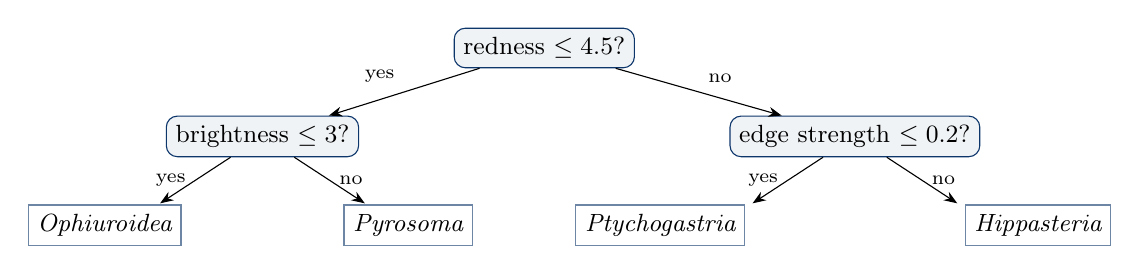
\begin{tikzpicture}[>=Stealth, font=\small, node distance=6mm and 4mm,
  q/.style={draw=ocean, rounded corners, fill=ocean!6, align=center},
  l/.style={draw=ocean!60, fill=white, align=center, font=\small\itshape}]
  \node[q] (r) {redness $\le 4.5$?};
  \node[q, below left=of r, xshift=-8mm] (a) {brightness $\le 3$?};
  \node[q, below right=of r, xshift=8mm] (b) {edge strength $\le 0.2$?};
  \node[l, below left=of a, xshift=6mm] {Ophiuroidea};
  \node[l, below right=of a, xshift=-6mm] {Pyrosoma};
  \node[l, below left=of b, xshift=6mm] {Ptychogastria};
  \node[l, below right=of b, xshift=-6mm] {Hippasteria};
  \draw[->] (r) -- node[above left, font=\scriptsize]{yes} (a);
  \draw[->] (r) -- node[above right, font=\scriptsize]{no} (b);
  \draw[->] (a) -- node[left, font=\scriptsize]{yes} +(-1.3,-0.85);
  \draw[->] (a) -- node[right, font=\scriptsize]{no} +(1.3,-0.85);
  \draw[->] (b) -- node[left, font=\scriptsize]{yes} +(-1.3,-0.85);
  \draw[->] (b) -- node[right, font=\scriptsize]{no} +(1.3,-0.85);
\end{tikzpicture}
\end{center}
Classify: (i) redness 6, brightness 2, edge strength 0.35; (ii) redness 3, brightness 7, edge strength 0.1; (iii) redness 4.5, brightness 2.5, edge strength 0.5.
\begin{solution}(i) $6 > 4.5$ $\rightarrow$ edge $0.35 > 0.2$ $\rightarrow$ \emph{Hippasteria}. (ii) $3 \le 4.5$ $\rightarrow$ brightness $7 > 3$ $\rightarrow$ \emph{Pyrosoma}. (iii) $4.5 \le 4.5$ $\rightarrow$ brightness $2.5 \le 3$ $\rightarrow$ \emph{Ophiuroidea}.\end{solution}
\answerspace{1.6cm}
\part[3] A colleague grows the tree until every leaf contains exactly one training crop. What happens to the training accuracy and to the test accuracy? Use the comparison with a taxonomist's key.
\begin{solution}Training accuracy becomes (nearly) 100\,\%, test accuracy usually drops: the tree overfits. It is like a key with one couplet per museum specimen -- it describes the individual specimens (and their noise) instead of the characters of the species, so new specimens fall into the wrong leaves.\end{solution}
\answerspace{2.1cm}
\end{parts}

% =====================================================================  D
\qbreak
\question \textbf{Interpreting an experiment.} The reference run of this course used CNN features (ResNet-18) and all \RefCrops\ crops, 79 labels, and three ways of splitting them into 75\,\% training and 25\,\% test crops (mean of 3 repetitions):
\begin{center}
\begin{tabular}{lcccc}
\toprule
 & \multicolumn{2}{c}{logistic regression} & \multicolumn{2}{c}{5-nearest neighbours} \\
split & train acc. & test acc. & train acc. & test acc. \\
\midrule
random (crop by crop) & \RefTrainLogregRandom & \RefRandomAcc & \RefTrainKnnRandom & \RefRandomAccKnn \\
image (crops of a frame together) & \RefTrainLogregImage & \RefImageAcc & \RefTrainKnnImage & \RefImageAccKnn \\
dive (crops of a dive together) & \RefTrainLogregDive & \RefDiveAcc & \RefTrainKnnDive & \RefDiveAccKnn \\
\bottomrule
\end{tabular}
\end{center}
In the random split, \RefSeenDiveRandom\ of the test crops come from a dive that also contributed training crops; in the dive split, 0\,\%.
\begin{parts}
\part[4] Describe the main result in two sentences.
\begin{solution}With the same features and classifier, test accuracy drops strongly from the random split (\RefRandomAcc) to the dive split (\RefDiveAcc), while training accuracy stays high. Keeping whole images together changes little; keeping whole dives together changes a lot.\end{solution}
\answerspace{2.1cm}
\part[6] Explain \emph{why} the accuracy depends on the split. Use what you know about how the images were recorded.
\begin{solution}Frames of one dive are recorded within hours at one site, with the same camera, light and background, and often show the same individual animal several times. In a random split near-identical crops land in training and test, so the classifier can ``recognise'' a crop it has practically seen (data leakage). In a dive split the test animals come from other places, other individuals, other conditions -- the classifier must really generalise.\end{solution}
\answerspace{3.1cm}
\part[3] $k$-NN profits more from the random split than logistic regression. Suggest a reason.
\begin{solution}$k$-NN labels a crop by its most similar training crops; with a random split these are often frames of the same individual from the same dive, so it effectively looks up a near-duplicate. Logistic regression learns one smooth weighted rule per label and relies less on individual training crops.\end{solution}
\answerspace{1.8cm}
\part[3] Which test accuracy belongs in a report about using the classifier on a future expedition? Justify.
\begin{solution}The dive-split number: a future expedition consists of new dives, so only a test on unseen dives estimates that situation; the random-split number is inflated by leakage.\end{solution}
\answerspace{1.8cm}
\part[4] A newspaper writes: ``AI identifies deep-sea animals with 98\,\% accuracy -- taxonomists no longer needed.'' Give two critical questions you would ask.
\begin{solution}Any two, e.g.: Was the 98\,\% measured on images from new dives/sites or on frames similar to the training images? Accuracy on which labels -- species or coarse groups, and how good is it on rare ones (balanced accuracy)? How severe are the remaining mistakes? Who labelled the test data -- are the labels themselves checked? Is it better than a sensible baseline? (The FathomNet winners: $\approx$98\,\% on training images but only 57--61\,\% on new dives.)\end{solution}
\answerspace{2.3cm}
\end{parts}

% =====================================================================  E
\qbreak
\question \textbf{Mistakes in the tree of life.}
\begin{center}
\small
\begin{tabular}{llllll}
\toprule
label & phylum & class & order & family & genus \\
\midrule
\emph{Sebastes diploproa} (species) & Chordata & Teleostei & Perciformes & Sebastidae & \emph{Sebastes} \\
\emph{Sebastes} (genus) & Chordata & Teleostei & Perciformes & Sebastidae & \emph{Sebastes} \\
\emph{Sebastolobus} (genus) & Chordata & Teleostei & Perciformes & Sebastidae & \emph{Sebastolobus} \\
Asteroidea (class) & Echinodermata & Asteroidea & & & \\
Ophiuroidea (class) & Echinodermata & Ophiuroidea & & & \\
Actiniaria (order) & Cnidaria & Hexacorallia & Actiniaria & & \\
\bottomrule
\end{tabular}
\end{center}
The \emph{tree distance} is the number of steps from the true label up to the lowest rank both labels share, plus the steps down to the predicted label (ranks: kingdom, phylum, class, order, family, genus, species).
\begin{parts}
\part[6] For each mistake give the lowest shared rank and the tree distance:
(i) truth \emph{Sebastes}, prediction \emph{Sebastes diploproa};
(ii) truth \emph{Sebastes diploproa}, prediction \emph{Sebastolobus};
(iii) truth Asteroidea, prediction Ophiuroidea;
(iv) truth Asteroidea, prediction Actiniaria.
\begin{solution}(i) genus \emph{Sebastes}: $0 + 1 = 1$. (ii) family Sebastidae: $2 + 1 = 3$ (species$\to$genus$\to$family, family$\to$genus). (iii) phylum Echinodermata: $1 + 1 = 2$. (iv) kingdom Animalia: $2 + 3 = 5$.\end{solution}
\answerspace{2.9cm}
\part[4] Mistake (i) is often not the classifier's fault. Explain why, and say what this means for how we should score such predictions.
\begin{solution}\emph{Sebastes diploproa} is a species inside the genus \emph{Sebastes}; a crop labelled \emph{Sebastes} may well show a \emph{S.\ diploproa} that the annotator could not identify to species. The prediction is then possibly correct but more specific than the label. A plain right/wrong score punishes this as hard as a cross-phylum error; a taxonomic distance (or scoring at genus rank) treats it as the small or non-mistake it is.\end{solution}
\answerspace{2.3cm}
\end{parts}

% =====================================================================  F
\qbreak
\question[10] \textbf{Design.} A research group wants to use a classifier to count animals in 200 hours of new ROV video from a seamount that has never been surveyed. They have the FathomNet training data. Describe in 6--10 bullet points how you would build, test and use the classifier responsibly.
\begin{solution}Credit for (about 1 point each, max.\ 10):
\begin{itemize}
\item Features from a pretrained CNN (transfer learning), classifier such as logistic regression; possibly fine-tune.
\item Split train/validation/test \textbf{by dive} (or by site/cruise); tune on validation only; test once.
\item Better still: annotate a small sample of the new seamount video by experts and test on it (new site, possibly new camera).
\item Compare with the majority baseline; report balanced accuracy / macro-F1, not only accuracy.
\item Per-label recall: find which taxa are unreliable; report those at a coarser rank or check by hand.
\item Look at mistake severity in the tree of life; report counts at the rank where the classifier is reliable (e.g.\ phylum/class).
\item Animals or labels not in the 79 training labels will be forced into a wrong label -- plan for ``unknown''.
\item Use the confidence: let experts check low-confidence predictions, and a random sample of confident ones (confident mistakes exist).
\item Look at mistakes with images; some are label errors; tiny/blurry crops are unreliable.
\item Document data, split, metrics and limitations; acknowledge FathomNet.
\end{itemize}\end{solution}
\answerspace{9.1cm}
\end{questions}
\end{document}
"   -> answer key
\documentclass[11pt,a4paper,addpoints]{exam}
\ifdefined\withsolutions\printanswers\fi
\usepackage[T1]{fontenc}
\usepackage{lmodern}
\usepackage[margin=2.2cm]{geometry}
\usepackage{booktabs, array, amsmath, xcolor, tikz, multirow}
\usetikzlibrary{arrows.meta, positioning}
% generated by write_numbers.py from results/reference_results.json - do not edit
\newcommand{\RefCrops}{23{,}664}
\newcommand{\RefDives}{1{,}465}
\newcommand{\RefTopTenDives}{21\,\%}
\newcommand{\RefTwoTrain}{444}
\newcommand{\RefTwoTest}{148}
\newcommand{\RefThr}{0.05}
\newcommand{\RefThrTrain}{98.4\,\%}
\newcommand{\RefThrTest}{98.0\,\%}
\newcommand{\RefCSPhylumMajority}{30.4\,\%}
\newcommand{\RefCSPhylumCentroid}{26.4\,\%}
\newcommand{\RefCSPhylumKnn}{55.0\,\%}
\newcommand{\RefCSPhylumTree}{50.3\,\%}
\newcommand{\RefCSLabelMajority}{1.3\,\%}
\newcommand{\RefCSLabelCentroid}{15.9\,\%}
\newcommand{\RefCSLabelKnn}{33.6\,\%}
\newcommand{\RefCSLabelTree}{23.7\,\%}
\newcommand{\RefCSLabelBest}{33.6\,\%}
\newcommand{\RefZooBestName}{neural network (MLP)}
\newcommand{\RefZooBest}{64.6\,\%}
\newcommand{\RefZooBestPixels}{46.3\,\%}
\newcommand{\RefZooBestColour}{48.4\,\%}
\newcommand{\RefZooRows}{majority baseline & 1.3\,\% & 1.3\,\% & $<$1\,s \\
nearest centroid & 39.9\,\% & 37.9\,\% & 2\,s \\
5-nearest neighbours & 69.9\,\% & 53.4\,\% & $<$1\,s \\
decision tree & 100.0\,\% & 20.5\,\% & 48\,s \\
random forest & 100.0\,\% & 56.1\,\% & 93\,s \\
logistic regression & 90.7\,\% & 63.7\,\% & 21\,s \\
neural network (MLP) & 92.4\,\% & 64.6\,\% & 13\,s \\}
\newcommand{\RefRandomAcc}{63.5\,\%}
\newcommand{\RefRandomAccKnn}{53.5\,\%}
\newcommand{\RefTrainLogregRandom}{90.7\,\%}
\newcommand{\RefTrainKnnRandom}{70.0\,\%}
\newcommand{\RefImageAcc}{57.5\,\%}
\newcommand{\RefImageAccKnn}{45.5\,\%}
\newcommand{\RefTrainLogregImage}{91.1\,\%}
\newcommand{\RefTrainKnnImage}{71.0\,\%}
\newcommand{\RefDiveAcc}{49.6\,\%}
\newcommand{\RefDiveAccKnn}{35.5\,\%}
\newcommand{\RefTrainLogregDive}{91.0\,\%}
\newcommand{\RefTrainKnnDive}{71.6\,\%}
\newcommand{\RefSeenDiveRandom}{97\,\%}
\newcommand{\RefRecallRows}{species & 33 & 67\,\% \\
genus & 21 & 69\,\% \\
family & 8 & 64\,\% \\
order & 6 & 56\,\% \\
class & 6 & 44\,\% \\
phylum & 1 & 27\,\% \\
other rank & 4 & 58\,\% \\}
\newcommand{\RefSevKingdom}{55\,\%}
\newcommand{\RefSevNear}{21\,\%}
\newcommand{\RefRandPhylumAcc}{80.0\,\%}
\newcommand{\RefDivePhylumAcc}{72.6\,\%}
\newcommand{\RefDiveFone}{0.475}
\newcommand{\RefDiveAccSingle}{49.8\,\%}

\definecolor{ocean}{HTML}{0D366B}
\renewcommand{\solutiontitle}{\noindent\textbf{\color{ocean}Model answer:}\enspace}
\SolutionEmphasis{\color{ocean!80!black}}
\shadedsolutions
\definecolor{SolutionColor}{HTML}{EAF2FC}
\pointsinrightmargin
% blank space for writing in the student version only; the answer key stays compact
\newcommand{\answerspace}[1]{\ifprintanswers\medskip\else\vspace{#1}\fi}
\newcommand{\qbreak}{\ifprintanswers\else\newpage\fi}
\bracketedpoints
\qformat{\textbf{Question \thequestion}\quad(\totalpoints\ points)\hfill}
\firstpageheader{Can a computer identify deep-sea animals?}{}{Final exam\ifprintanswers\ -- \textbf{ANSWER KEY}\fi}
\runningheader{}{}{Final exam\ifprintanswers\ -- answer key\fi}
\firstpagefooter{}{Page \thepage\ of \numpages}{}
\runningfooter{}{Page \thepage\ of \numpages}{}

\begin{document}
\begin{center}
{\LARGE\bfseries Final exam}\\[4pt]
{\large Can a computer identify deep-sea animals? -- A classifier project with FathomNet 2025}\\[10pt]
\end{center}

\noindent\begin{tabular}{@{}p{0.55\textwidth}p{0.4\textwidth}@{}}
Name: \hrulefill & Student ID: \hrulefill \\
\end{tabular}

\vspace{8pt}
\noindent\textbf{Time:} 90 minutes. \textbf{Allowed:} pocket calculator, one handwritten A4 sheet (both sides).
Answer in the space provided; short, precise answers are best. Give one decimal place for percentages.
There are \numpoints\ points in total.

\begin{center}
\gradetable[h][questions]
\end{center}

\begin{questions}

% =====================================================================  A
\question \textbf{Concepts.} Answer each part in one or two sentences.
\begin{parts}
\part[2] What is the difference between the \emph{training set} and the \emph{test set}?
\begin{solution}The training set is the set of labelled examples the classifier learns its rule from. The test set holds other labelled examples that are used only to measure how well the finished rule works on specimens it has not seen.\end{solution}
\answerspace{1.8cm}

\part[2] What is a \emph{feature}? Give two examples of features used in this course.
\begin{solution}A number that describes an object and is given to the classifier (like a character in a key). Examples: redness, brightness, edge strength, a pixel value, one of the 512 CNN embedding numbers.\end{solution}
\answerspace{1.8cm}

\part[2] Why is the accuracy on the training set not a good measure of how good a classifier is?
\begin{solution}A flexible classifier can memorise the training examples (e.g.\ 1-NN is always 100\,\% right on them). Training accuracy measures memory, not the ability to label new specimens; flexible rules can overfit.\end{solution}
\answerspace{1.8cm}

\part[2] There are 79 labels, each with the same number of test crops. What accuracy does the \emph{majority baseline} reach, and why is this number useful?
\begin{solution}$1/79 \approx 1.3\,\%$. Any real classifier must beat it; it tells you what ``no skill'' looks like (the baseline is much higher when labels are imbalanced or there are few of them).\end{solution}
\answerspace{1.8cm}

\part[2] Which classifier corresponds to a dichotomous identification key, and which to ``compare the specimen with the most similar ones in the reference collection''?
\begin{solution}Decision tree $=$ key; $k$-nearest neighbours $=$ comparing with the reference collection.\end{solution}
\answerspace{1.6cm}

\part[2] What does \emph{transfer learning} mean in this course?
\begin{solution}We used a CNN that was trained on a different task (ImageNet everyday photos) as a ready-made feature extractor for deep-sea crops, and trained only a simple classifier on its 512 output numbers.\end{solution}
\answerspace{1.8cm}

\part[2] What is the \emph{validation set} used for, and why must the test set not be used for the same purpose?
\begin{solution}For choosing between ideas/settings (features, classifier, $k$ \dots). If we chose on the test set, we would pick the idea that was lucky on those test crops and the reported score would be too optimistic.\end{solution}
\answerspace{1.8cm}

\part[2] Before using $k$-nearest neighbours we \emph{standardise} the features (each feature gets mean 0 and standard deviation 1). Why?
\begin{solution}$k$-NN uses distances. Without standardisation, a feature with large numbers (e.g.\ a value 0--255) dominates the distance and features with small ranges (0--1) are effectively ignored.\end{solution}
\answerspace{1.8cm}

\part[2] For the label \emph{Asteroidea} the classifier has high recall but low precision. Describe in words what it does.
\begin{solution}It finds almost all real sea stars, but it also calls many other animals ``Asteroidea'' -- many of its Asteroidea predictions are wrong.\end{solution}
\answerspace{1.8cm}

\part[2] Give two reasons why a label at a high rank (e.g.\ the class \emph{Asteroidea}) is harder to learn than a species label.
\begin{solution}(1) It covers many different-looking species, so its crops are very variable. (2) Experts use coarse labels exactly when the animal is hard to see (small, blurry, partly hidden), so the crops are of lower quality. (Also: it overlaps visually with its own lower-rank labels.)\end{solution}
\answerspace{1.8cm}
\end{parts}

% =====================================================================  B
\qbreak
\question \textbf{Accuracy, precision, recall.} A classifier was tested on 100 crops of three labels. Rows are the \emph{true} labels, columns the \emph{predicted} labels.
\begin{center}
\begin{tabular}{ll|ccc|c}
\toprule
 & & \multicolumn{3}{c|}{\textbf{predicted}} & \\
 & & Asteroidea & Ophiuroidea & Actiniaria & total \\
\midrule
\multirow{3}{*}{\textbf{true}} & Asteroidea (sea stars) & 40 & 8 & 2 & 50 \\
 & Ophiuroidea (brittle stars) & 10 & 25 & 5 & 40 \\
 & Actiniaria (sea anemones) & 0 & 5 & 5 & 10 \\
\midrule
 & total & 50 & 38 & 12 & 100 \\
\bottomrule
\end{tabular}
\end{center}
\begin{parts}
\part[3] Compute the accuracy.
\begin{solution}$(40+25+5)/100 = 70.0\,\%$.\end{solution}
\answerspace{1.3cm}
\part[6] Compute the recall of each label and the balanced accuracy.
\begin{solution}Asteroidea $40/50 = 80.0\,\%$; Ophiuroidea $25/40 = 62.5\,\%$; Actiniaria $5/10 = 50.0\,\%$. Balanced accuracy $= (80.0+62.5+50.0)/3 = 64.2\,\%$.\end{solution}
\answerspace{2.1cm}
\part[4] Compute the precision of \emph{Actiniaria} and of \emph{Ophiuroidea}.
\begin{solution}Actiniaria: $5/12 = 41.7\,\%$. Ophiuroidea: $25/38 = 65.8\,\%$.\end{solution}
\answerspace{1.6cm}
\part[3] What accuracy and what balanced accuracy would the majority baseline reach on these 100 crops?
\begin{solution}It always predicts Asteroidea: accuracy $50/100 = 50.0\,\%$; recalls 100, 0, 0\,\% $\Rightarrow$ balanced accuracy $33.3\,\%$.\end{solution}
\answerspace{1.6cm}
\part[4] Asteroidea and Ophiuroidea are both Echinodermata; Actiniaria are Cnidaria. How many of the 30 mistakes stay within the correct phylum? Which kind of mistake is worse for a biodiversity survey, and why?
\begin{solution}Within Echinodermata: $8 + 10 = 18$ of 30 (60\,\%); the other 12 confuse phyla. A cross-phylum mistake is worse: it puts the animal in a completely different part of the tree of life (different body plan, ecology, feeding), so higher-rank summaries (e.g.\ ``number of echinoderms'') become wrong too; a within-phylum mistake still gives correct counts at phylum level.\end{solution}
\answerspace{2.1cm}
\end{parts}

% =====================================================================  C
\qbreak
\question \textbf{Classifiers by hand.}
Six training crops are described by two standardised features (redness, brightness):
\begin{center}
\begin{tabular}{cccl}
\toprule
crop & redness & brightness & label \\
\midrule
1 & 2 & 8 & \emph{Pyrosoma} (tunicate) \\
2 & 1 & 6 & \emph{Pyrosoma} \\
3 & 3 & 5 & \emph{Pyrosoma} \\
4 & 7 & 4 & \emph{Ptychogastria} (jellyfish) \\
5 & 8 & 7 & \emph{Ptychogastria} \\
6 & 6 & 2 & \emph{Ptychogastria} \\
\bottomrule
\end{tabular}
\end{center}
A new crop $X$ has redness 5 and brightness 5.
\begin{parts}
\part[6] Compute the Euclidean distance from $X$ to each training crop
\\ \hspace*{1.5em}$d = \sqrt{(\Delta\,\text{redness})^2 + (\Delta\,\text{brightness})^2}$
\begin{solution}1: $\sqrt{9+9}=4.24$; 2: $\sqrt{16+1}=4.12$; 3: $\sqrt{4+0}=2.00$; 4: $\sqrt{4+1}=2.24$; 5: $\sqrt{9+4}=3.61$; 6: $\sqrt{1+9}=3.16$.\end{solution}
\answerspace{2.6cm}
\part[4] Classify $X$ with $k$-NN for $k = 1$ and for $k = 3$. Why can the two answers differ?
\begin{solution}$k=1$: nearest is crop 3 $\Rightarrow$ \emph{Pyrosoma}. $k=3$: crops 3 (P), 4 (J), 6 (J) $\Rightarrow$ \emph{Ptychogastria} (2:1). A single neighbour can be an unusual specimen; a vote over more neighbours smooths the boundary (less sensitive to single crops, less overfitting).\end{solution}
\answerspace{2.1cm}
\part[4] Classify $X$ with the nearest-centroid classifier. Show the two centroids.
\begin{solution}Centroid \emph{Pyrosoma} $=(2,\ 6.33)$, \emph{Ptychogastria} $=(7,\ 4.33)$. Distances: $\sqrt{9+1.78}=3.28$ and $\sqrt{4+0.44}=2.11$ $\Rightarrow$ \emph{Ptychogastria}.\end{solution}
\answerspace{2.1cm}
\part[3] A decision tree learned from crops of four labels:
\begin{center}
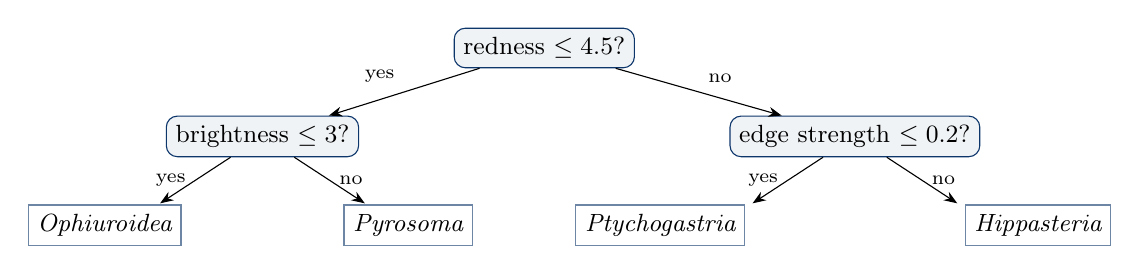
\begin{tikzpicture}[>=Stealth, font=\small, node distance=6mm and 4mm,
  q/.style={draw=ocean, rounded corners, fill=ocean!6, align=center},
  l/.style={draw=ocean!60, fill=white, align=center, font=\small\itshape}]
  \node[q] (r) {redness $\le 4.5$?};
  \node[q, below left=of r, xshift=-8mm] (a) {brightness $\le 3$?};
  \node[q, below right=of r, xshift=8mm] (b) {edge strength $\le 0.2$?};
  \node[l, below left=of a, xshift=6mm] {Ophiuroidea};
  \node[l, below right=of a, xshift=-6mm] {Pyrosoma};
  \node[l, below left=of b, xshift=6mm] {Ptychogastria};
  \node[l, below right=of b, xshift=-6mm] {Hippasteria};
  \draw[->] (r) -- node[above left, font=\scriptsize]{yes} (a);
  \draw[->] (r) -- node[above right, font=\scriptsize]{no} (b);
  \draw[->] (a) -- node[left, font=\scriptsize]{yes} +(-1.3,-0.85);
  \draw[->] (a) -- node[right, font=\scriptsize]{no} +(1.3,-0.85);
  \draw[->] (b) -- node[left, font=\scriptsize]{yes} +(-1.3,-0.85);
  \draw[->] (b) -- node[right, font=\scriptsize]{no} +(1.3,-0.85);
\end{tikzpicture}
\end{center}
Classify: (i) redness 6, brightness 2, edge strength 0.35; (ii) redness 3, brightness 7, edge strength 0.1; (iii) redness 4.5, brightness 2.5, edge strength 0.5.
\begin{solution}(i) $6 > 4.5$ $\rightarrow$ edge $0.35 > 0.2$ $\rightarrow$ \emph{Hippasteria}. (ii) $3 \le 4.5$ $\rightarrow$ brightness $7 > 3$ $\rightarrow$ \emph{Pyrosoma}. (iii) $4.5 \le 4.5$ $\rightarrow$ brightness $2.5 \le 3$ $\rightarrow$ \emph{Ophiuroidea}.\end{solution}
\answerspace{1.6cm}
\part[3] A colleague grows the tree until every leaf contains exactly one training crop. What happens to the training accuracy and to the test accuracy? Use the comparison with a taxonomist's key.
\begin{solution}Training accuracy becomes (nearly) 100\,\%, test accuracy usually drops: the tree overfits. It is like a key with one couplet per museum specimen -- it describes the individual specimens (and their noise) instead of the characters of the species, so new specimens fall into the wrong leaves.\end{solution}
\answerspace{2.1cm}
\end{parts}

% =====================================================================  D
\qbreak
\question \textbf{Interpreting an experiment.} The reference run of this course used CNN features (ResNet-18) and all \RefCrops\ crops, 79 labels, and three ways of splitting them into 75\,\% training and 25\,\% test crops (mean of 3 repetitions):
\begin{center}
\begin{tabular}{lcccc}
\toprule
 & \multicolumn{2}{c}{logistic regression} & \multicolumn{2}{c}{5-nearest neighbours} \\
split & train acc. & test acc. & train acc. & test acc. \\
\midrule
random (crop by crop) & \RefTrainLogregRandom & \RefRandomAcc & \RefTrainKnnRandom & \RefRandomAccKnn \\
image (crops of a frame together) & \RefTrainLogregImage & \RefImageAcc & \RefTrainKnnImage & \RefImageAccKnn \\
dive (crops of a dive together) & \RefTrainLogregDive & \RefDiveAcc & \RefTrainKnnDive & \RefDiveAccKnn \\
\bottomrule
\end{tabular}
\end{center}
In the random split, \RefSeenDiveRandom\ of the test crops come from a dive that also contributed training crops; in the dive split, 0\,\%.
\begin{parts}
\part[4] Describe the main result in two sentences.
\begin{solution}With the same features and classifier, test accuracy drops strongly from the random split (\RefRandomAcc) to the dive split (\RefDiveAcc), while training accuracy stays high. Keeping whole images together changes little; keeping whole dives together changes a lot.\end{solution}
\answerspace{2.1cm}
\part[6] Explain \emph{why} the accuracy depends on the split. Use what you know about how the images were recorded.
\begin{solution}Frames of one dive are recorded within hours at one site, with the same camera, light and background, and often show the same individual animal several times. In a random split near-identical crops land in training and test, so the classifier can ``recognise'' a crop it has practically seen (data leakage). In a dive split the test animals come from other places, other individuals, other conditions -- the classifier must really generalise.\end{solution}
\answerspace{3.1cm}
\part[3] $k$-NN profits more from the random split than logistic regression. Suggest a reason.
\begin{solution}$k$-NN labels a crop by its most similar training crops; with a random split these are often frames of the same individual from the same dive, so it effectively looks up a near-duplicate. Logistic regression learns one smooth weighted rule per label and relies less on individual training crops.\end{solution}
\answerspace{1.8cm}
\part[3] Which test accuracy belongs in a report about using the classifier on a future expedition? Justify.
\begin{solution}The dive-split number: a future expedition consists of new dives, so only a test on unseen dives estimates that situation; the random-split number is inflated by leakage.\end{solution}
\answerspace{1.8cm}
\part[4] A newspaper writes: ``AI identifies deep-sea animals with 98\,\% accuracy -- taxonomists no longer needed.'' Give two critical questions you would ask.
\begin{solution}Any two, e.g.: Was the 98\,\% measured on images from new dives/sites or on frames similar to the training images? Accuracy on which labels -- species or coarse groups, and how good is it on rare ones (balanced accuracy)? How severe are the remaining mistakes? Who labelled the test data -- are the labels themselves checked? Is it better than a sensible baseline? (The FathomNet winners: $\approx$98\,\% on training images but only 57--61\,\% on new dives.)\end{solution}
\answerspace{2.3cm}
\end{parts}

% =====================================================================  E
\qbreak
\question \textbf{Mistakes in the tree of life.}
\begin{center}
\small
\begin{tabular}{llllll}
\toprule
label & phylum & class & order & family & genus \\
\midrule
\emph{Sebastes diploproa} (species) & Chordata & Teleostei & Perciformes & Sebastidae & \emph{Sebastes} \\
\emph{Sebastes} (genus) & Chordata & Teleostei & Perciformes & Sebastidae & \emph{Sebastes} \\
\emph{Sebastolobus} (genus) & Chordata & Teleostei & Perciformes & Sebastidae & \emph{Sebastolobus} \\
Asteroidea (class) & Echinodermata & Asteroidea & & & \\
Ophiuroidea (class) & Echinodermata & Ophiuroidea & & & \\
Actiniaria (order) & Cnidaria & Hexacorallia & Actiniaria & & \\
\bottomrule
\end{tabular}
\end{center}
The \emph{tree distance} is the number of steps from the true label up to the lowest rank both labels share, plus the steps down to the predicted label (ranks: kingdom, phylum, class, order, family, genus, species).
\begin{parts}
\part[6] For each mistake give the lowest shared rank and the tree distance:
(i) truth \emph{Sebastes}, prediction \emph{Sebastes diploproa};
(ii) truth \emph{Sebastes diploproa}, prediction \emph{Sebastolobus};
(iii) truth Asteroidea, prediction Ophiuroidea;
(iv) truth Asteroidea, prediction Actiniaria.
\begin{solution}(i) genus \emph{Sebastes}: $0 + 1 = 1$. (ii) family Sebastidae: $2 + 1 = 3$ (species$\to$genus$\to$family, family$\to$genus). (iii) phylum Echinodermata: $1 + 1 = 2$. (iv) kingdom Animalia: $2 + 3 = 5$.\end{solution}
\answerspace{2.9cm}
\part[4] Mistake (i) is often not the classifier's fault. Explain why, and say what this means for how we should score such predictions.
\begin{solution}\emph{Sebastes diploproa} is a species inside the genus \emph{Sebastes}; a crop labelled \emph{Sebastes} may well show a \emph{S.\ diploproa} that the annotator could not identify to species. The prediction is then possibly correct but more specific than the label. A plain right/wrong score punishes this as hard as a cross-phylum error; a taxonomic distance (or scoring at genus rank) treats it as the small or non-mistake it is.\end{solution}
\answerspace{2.3cm}
\end{parts}

% =====================================================================  F
\qbreak
\question[10] \textbf{Design.} A research group wants to use a classifier to count animals in 200 hours of new ROV video from a seamount that has never been surveyed. They have the FathomNet training data. Describe in 6--10 bullet points how you would build, test and use the classifier responsibly.
\begin{solution}Credit for (about 1 point each, max.\ 10):
\begin{itemize}
\item Features from a pretrained CNN (transfer learning), classifier such as logistic regression; possibly fine-tune.
\item Split train/validation/test \textbf{by dive} (or by site/cruise); tune on validation only; test once.
\item Better still: annotate a small sample of the new seamount video by experts and test on it (new site, possibly new camera).
\item Compare with the majority baseline; report balanced accuracy / macro-F1, not only accuracy.
\item Per-label recall: find which taxa are unreliable; report those at a coarser rank or check by hand.
\item Look at mistake severity in the tree of life; report counts at the rank where the classifier is reliable (e.g.\ phylum/class).
\item Animals or labels not in the 79 training labels will be forced into a wrong label -- plan for ``unknown''.
\item Use the confidence: let experts check low-confidence predictions, and a random sample of confident ones (confident mistakes exist).
\item Look at mistakes with images; some are label errors; tiny/blurry crops are unreliable.
\item Document data, split, metrics and limitations; acknowledge FathomNet.
\end{itemize}\end{solution}
\answerspace{9.1cm}
\end{questions}
\end{document}
